%
% Шаблон для НИР
%

\documentclass[a4paper,12pt]{article}
\usepackage[backend=biber,sorting=none,style=gost-numeric,autolang=other]{biblatex} % библиография
\usepackage{mathtext} %русские буквы в формулах
\usepackage[T2A]{fontenc}
\usepackage[utf8]{inputenc}
\usepackage[english,russian]{babel}
\usepackage{amsmath}
\usepackage{fancyvrb}
\usepackage{formular}
\usepackage{setspace} % управление междустрочными интервалами
%поля документа
\usepackage[left=3cm,right=1cm,top=2cm,bottom=2cm]{geometry}
%\usepackage{csquotes}
\usepackage{misccorr} % точки в конце номеров разделов, использовать перед пакетом ccaption!
\usepackage{ccaption} % изменения подписей к рисункам и табл.
% отступ перед первым абзацем
\usepackage{indentfirst}
%вставка изображений
\usepackage{graphicx}
% счетчики
\usepackage{totcount}
% управление содержанием
\usepackage{tocloft}
% управление таблицами и рисунками
\usepackage{float}

%\hfill

%для добавления количества источников в реферат
\newtotcounter{citnum} %From the package documentation
\def\oldbibitem{} \let\oldbibitem=\bibitem
\def\bibitem{\stepcounter{citnum}\oldbibitem}

% окружение для листингов - с нумерацией строк слева
\DefineVerbatimEnvironment{MyCode}{Verbatim}{frame=lines,numbers=left,numberblanklines=false,framesep=5mm}

% автоматическая нумерация листингов
\newfloat{Program}{phb}{lop}
\floatname{Program}{Листинг}
\floatstyle{ruled}

\setcounter{secnumdepth}{3} % глубина нумерации до подразделов

%если нужны точки в оглавлении для разделов - раскомментируйте следующую команду
%\renewcommand{\cftsecleader}{\cftdotfill{\cftdotsep}}

\addto\captionsrussian{%
\renewcommand{\figurename}{Рисунок}%
%\renewcommand{\tablename}{Таблица}%
}

% дефис в подписи к рисункам
\captiondelim{ -- } 

% Настройки для окружений с подчеркиваниями для подписей и пр.
\setFRMfontencoding{T2A}
\setFRMdfontencoding{T2A}
% thanks to A.Starikov
\setFRMfontfamily{cmr}
\setFRMdfontfamily{ptm}
\setFRMdfontsize{10pt}

% задает длину поля для подписи на титульной странице
\newFRMfield{xtitlesign}{40mm}

% поле для факультета или кафедры
\newFRMfield{fcath}{65mm}


\addbibresource{rbiblio.bib}

\begin{document}

% счетчики страниц, рисунков, таблиц
\regtotcounter{page}
\regtotcounter{figure}
\regtotcounter{table}

\renewcommand{\refname}{\centerline{СПИСОК ИСПОЛЬЗОВАННОЙ ЛИТЕРАТУРЫ}} 
\renewcommand{\contentsname}{\centerline{СОДЕРЖАНИЕ}} 
%\renewcommand{\refname}{Список источников}  % По умолчанию "Список литературы" (article)
%\renewcommand{\bibname}{Литература}  % По умолчанию "Литература" (book и report)

% титульная страница
\thispagestyle{empty}
\begin{center} \small
\textbf{МИНИСТЕРСТВО ОБРАЗОВАНИЯ И НАУКИ РОССИЙСКОЙ ФЕДЕРАЦИИ}\\
ФЕДЕРАЛЬНОЕ ГОСУДАРСТВЕННОЕ АВТОНОМНОЕ ОБРАЗОВАТЕЛЬНОЕ УЧРЕЖДЕНИЕ
ВЫСШЕГО  ОБРАЗОВАНИЯ\\
«Национальный исследовательский ядерный университет «МИФИ»\\
\textbf{Обнинский институт атомной энергетики} – \\
филиал федерального государственного автономного образовательного учреждения высшего\\
образования «Национальный исследовательский ядерный университет «МИФИ»\\
(ИАТЭ НИЯУ МИФИ)
\end{center}
%\vfill
\medskip

% Направление подготовки следует уточнять,
% магистры и бакалавры могут иметь разные наименования
\begin{center}
\begin{tabular}{rl}
	
Отделение & \useFRMfield{fcath}[\large Интеллектуальных кибернетических систем] \\ 
Направление подготовки & \useFRMfield{fcath}[\large Информационные системы и технологии] \\ 
\end{tabular} 
\end{center}

\vfill

\large 

\begin{center}
	Научно-исследовательская работа \\
	
	\medskip
	
	\textbf{\Large 
		Разработка мобильного приложения для преобразования 2D фотографий в 3D вид
	}
\end{center}

\vspace{1cm}

\begin{tabular*}{\textwidth}{lcr}
Студент группы ИС-Б14 & \useFRMfield{xtitlesign} & А.В.Кузнецов\\
& & \\
Руководитель & & \\
к.т.н., доцент отделения ИКС & \useFRMfield{xtitlesign} & О.А.Мирзеабасов
\end{tabular*}


\vfill
\large

\begin{center}
Обнинск, 2017
\end{center}

\onehalfspacing

\pagebreak

% реферат
%\thispagestyle{empty}

\section*{\centering РЕФЕРАТ}

% возможно, кол-во источников придется вставлять вручную
\total{page} стр., \total{table} табл., \total{figure} рис. , 5 ист. 

ANDROID, МОБИЛЬНОЕ ПРИЛОЖЕНИЕ, ПОЛЬЗОВАТЕЛЬСКИЙ ИНТЕРФЕЙС, UI/UX, КАРТА ГЛУБИНЫ, АНАЛИЗ, 3D, АНИМАЦИЯ, GIF 

Настоящая работа посвящена изучению методов получения трехмерных изображений из двумерных и разработке пользовательского интерфейса мобильного приложения для преобразования 2D фотографий в 3D вид. 

\pagebreak
\thispagestyle{empty}

\section*{\centering ОБОЗНАЧЕНИЯ И СОКРАЩЕНИЯ}

\noindent
UI (user interface) --- пользовательский интерфейс\\
UX (user experience) --- пользовательский опыт\\
Референсы --- изображения или другие ресурсы для разработки графического интерфейса с учетом существующих, успешно работающих решений

\pagebreak



\tableofcontents
% если нужно добавить "Стр." над номерами страниц - раскомментируйте следующую команду
%\addtocontents{toc}{~\hfill\textbf{Стр.}\par}

\pagebreak

\section*{\centering ВВЕДЕНИЕ}
\addcontentsline{toc}{section}{ВВЕДЕНИЕ}

Основным результатом выполнения проекта будет мобильное приложение, предназначенное для преобразования 2D изображений в 3D вид. Приложение будет распространяться с помощью его размещения в Google Play (для Android-устройств). Соответственно, в качестве основных потребителей создаваемой продукции следует рассматривать владельцев мобильных устройств, которые любят использовать свой телефон или планшет в качестве фотоаппарата. Более того, то подмножество этих пользователей, которые, помимо фотографирования, активно обрабатывают свои фото средствами мобильного устройства и активно делятся этими результатами с друзьями посредством соцсетей.

Поэтому главной целью текущей НИР является исследованию	преобразования двумерных изображений в трехмерные и разработке современного, функционального и удобного пользовательского интерфейса. 

Задачи, решаемые в ходе работы (в соответствии с заданием на НИР):
\begin{enumerate}
    \item Изучение метода «дефокусировки» и семантического анализа;
    \item Разработка концепции и архитектуры мобильных приложений, предназначенных для преобразования 2D в 3D;
    \item Анализ существующих продуктов со схожим функционалом;
    \item Подготовка отчета и презентации по НИР.
\end{enumerate}
 % текст введения в файле intro.tex
\pagebreak

%\input{Post_zad}
\pagebreak
% первая глава

\section{Методы получения трехмерных изображений из двумерных}

В ходе выполнения проекта, главным образом, решается задача преобразования двумерных изображений в трехмерные на мобильных устройствах.

В последние годы заметное место в области преобразования и фильтрации изображений занимает задача преобразования двумерных изображений в трехмерные. На сегодняшний день в мире для этого разработаны различные методики, которые позволяют автоматически создавать так называемые «карты глубины»\cite{depthMap3} для двумерных изображений, основываясь на свойствах этого изображение и на некоторых предположениях о характере сцены.  В частности, были проведены исследования следующих методов получения трехмерных изображений из двумерных:

\begin{itemize}
	\item Предположение о том, что изображение имеет линейную перспективу;
	\item Предположение о том, что снимок сделан на открытом пространстве и использование модели рассеяния световых лучей в атмосфере;
	\item Обнаружение теней и восстановление по ним карты глубины;
	\item Обнаружение перекрытий объектов на изображении и используя эту информацию восстановлении карты глубины;
	\item Использование моделей пространственных искажений заданных текстур;
	\item Использование билатеральных симметричных шаблонов;
	\item Использование статистических методов для обучения текстурных шаблонов, на различных расстояниях от объектива и другие методы.
\end{itemize}

Практически все эти методы характеризуются достаточно узким характером сцен, которые могут быть реализованы для преобразования в трехмерное изображение. 

Проведенные предварительные исследования показали, что одним из наиболее перспективных методов преобразования изображений в трехмерные считается метод «дефокусировки», который предполагает, что близкие объекты находятся в фокусе, а более удаленные объекты имеют большее размытие. Используя информацию о размытии той или иной точки на изображении можно предположить о том, насколько далеко она находится от объектива.  Используя метод дефокусировки можно построить карту глубины для любой макрофотографии. 

Известные методы получения карты глубины использующие дефокус удаленных от объектива объектов основана на следующей цепочке преобразования изображения\cite{depthMap1}:

\begin{enumerate} 
	\item Обнаружение краев объектов с использованием фильтра Канни.
	\item Для каждой точки найденного края выполняется оценка расстояния, до нее с использованием гауссовского размытия. Таким образом строится так называемая разреженная карта глубины, которая несет информацию о расстоянии до объектива в некоторых точках изображения. 
	\item Разреженная карта глубины с использованием интерполяции превращается в так называемую «плотную карту глубины», которая уже пригодна для построения трехмерного изображения сцены с любого ракурса. 
\end{enumerate}

Реализация мобильного приложения позволяющего оперативно переводить стандартные фотоизображения в 3D-снимки чрезвычайно актуально и востребовано.  С другой стороны, на сегодняшний день имеется определенный научный задел по разработке алгоритмов преобразования 2D -3D. В частности известен ряд различных методик, которые позволяют автоматически создавать «карты глубины» для двумерных изображений, основываясь на свойствах этого изображение, и на некоторых предположениях о характере сцены. Например метод дефокусировки позволяет  построить карту глубины фотографии. Вместе с тем информации о программно реализованных в том числе мобильных приложений крайне мало. 

Рассмотренный метод преобразования (см. пункты 1-3) предыдущего раздела страдает двумя существенными недостатками\cite{depthMap2}.

\begin{enumerate}
	\item Разреженная карта глубины получается не всегда гладкой, что приводит к ошибкам последующей интерполяции и, в итоге, к ошибкам в карте глубины. 
	\item Окончательная интерполяция для построения требует больших вычислительных затрат и до последнего времени не имела возможности быть встроенной в мобильные приложения. 
\end{enumerate}

Основываясь на этих двух недостатках существующего метода дефокусировки изображения, требуется провести научное исследование в следующих направлениях:

\begin{enumerate}
	\item Адаптивное сглаживание разреженной карты глубины.  С использованием методов кластеризации краев изображения, в протяженные структуры, глубина точек которых должна подчиняться некоторому закону, а не быть случайной от точки к точке, как в существующем методе. 
	\item Найти способ снижения вычислительных затрат для выполнения двумерной интерполяции при построении плотной карты глубины. 
	\item Нам представляется, что для преобразования двумерного видеоролика в трехмерное представление необходимо разработать методику передачи разреженной карты глубины (с учетом сглаживания) от кадра к кадру. 
\end{enumerate}

Таким образом предлагаемый Проект на сегодняшний день актуален и содержит помимо научной алгоритмической составляющей широкие перспективы коммерциализации.

\section{Технические требования.}

В ходе выполнения проекта будет создана методика количественной оценки достоверности построения карты глубины, которая необходима для корректного преобразования 2D изображения в 3D вид. Эта методика основана на сравнении показаний глубины, полученных в результате работы алгоритмов преобразования 2D –> 3D и достоверных показаний глубины для данной сцены, которые получены в ручном режиме.

Для реализации методики предполагается произвести ручную разметку тестовых цифровых фотографий в количестве не менее 100 штук. Для этого в ручном режиме устанавливаются контрольные точки, с указанием расстояния до них.

Таким образом формируется разреженная карта глубины, с указанием абсолютных значений. Далее, на изображении находится самая дальняя контрольная точка и все расстояния нормируются на расстояние до нее. Таким образом формируется разреженная карта глубины с относительными расстояниями, и, как следствие, (алгоритмически) формируется «эталонная» плотная карта глубины.

Далее, в результате работы различных алгоритмов преобразования изображения из двумерного в трехмерное автоматически вычисляется как разреженная карта глубины для каждого из анализируемых алгоритмов (создаваемого в рамках проекта и конкурирующих аналогов). Далее предполагается вычислять среднеквадратичную ошибку между эталонными значениями для карты глубины и значениями, вычисленными каждым из алгоритмов.

Предполагается, что алгоритм, реализуемый в ходе выполнения проекта даст снижение такой ошибки между вычисленными и эталонными значениями на величину не менее 25\% (ожидаемое значение – порядка 30\%).

Необходимая задача при реализации проекта - адаптация существующего метода преобразования 2D в 3D для использования под управлением операционной системы Android.

В ходе выполнения проекта будут созданы мобильные приложения со следующими характеристиками:

\begin{itemize}
	\item мобильное приложение, функционирующее под управлением операционной системы Android версии не ниже 5.0.
	\item специальных дополнительных требований к аппаратному обеспечению мобильных устройств не предъявляется. Они соответствуют требованиям, накладываемым вышеперечисленными версиями ОС.
	\item мобильные приложения должны функционировать на устройствах с разными размерами экрана от 2.6 до 6 дюймов с разрешениями от 240х320 до 1440х2560 пикселей.
	\item источник данных для конвертирования - файлы в формате jpeg из галереи мобильного устройства или фотография, сделанная штатной фотокамерой мобильного устройства.
	\item мобильные приложения должны обеспечивать конвертацию сделанных фотокамерой изображений при максимальном качестве съемки не менее 10 Мп.
	\item формат данных, в которых сохраняются результаты - анаглиф файлы (формат jpeg), стерео пара (формат jps), анимированные файлы в формате gif.
	\item ориентировочное время преобразования 2D в 3D не должно превышать 5 секунд.
\end{itemize}

Основные технические параметры, определяющие количественные, качественные характеристики:

\begin{itemize}
\item 3D режим фотосъемки.
\item 3D режим видеосъёмки. 
\item Цифровая стабилизация изображения.
\item Передача файлов в формате Stereo JPEG (*.jps) на внешние устройства. 
\item Отображение файлов в формате Stereo JPEG (*.jps) на мобильном устройстве. 
\item Время преобразования цифровой фотографии в стереоизображение JPEG (*.jps) не превышает 5ти секунд. 
\item Возможность преобразования любой цифровой фотографии из галереи телефона в формат Stereo JPEG (*.jps)
\end{itemize}

\subsection{Технологические требования}

Создаваемое в рамках проекта мобильное приложение должно
функционировать под управлением мобильных операционных систем Android.

\begin{itemize}
	\item Программное обеспечение должно создаваться в строгом соответствии с модульным принципом.
	\item Программное обеспечение должно быть реализовано в виде "нативных" приложений для вышеперечисленных операционных систем.
	\item Ожидаемое время преобразования цифровой фотографии в трехмерный вид не должно превышать 5ти секунд. 
\end{itemize}

Технические требования к аппаратному обеспечению мобильного устройства и ограничения, накладываемые на преобразуемые фотографии, будут уточнены в ходе выполнения проекта.

\section{Разработка концепции и архитектуры мобильных приложений, предназначенных для преобразования 2D в 3D.}


\section{Анализ аналогичных приложений}
Одной из задач при создании мобильного приложения для преобразования 2D фотографий в 3D вид, является разработка пользовательского интерфейса.

Для достижения этой задачи были проанализированы аналогичные приложения, которые очень популярны на сегодняшний день: Prisma, Pixlr, Candy Camera.

В первую очередь, целью сравнения являлся анализ особенностей пользовательского интерфейса этих приложений. Это обусловлено тем, что, во многом, схема функционирования приложения, которое планируется создать в ходе выполнения проекта, аналогична схеме работы этих приложений. А именно: пользователь делает фотографию при помощи штатной камеры своего смартфона или загружает уже существующее изображение из галереи, отправляет изображение на обработку, просматривает результат и, если результат ему нравится, сохраняет или отправляет получившееся изображение в одну или несколько социальных сетей.

Таким образом можно выделить 4 основных окна приложения:
\begin{enumerate}
	\item Режим камеры, делаем фотографию.
	\item Окно выбора фотографии из галереи.
	\item Окно применения фильтра, смотрим готовый результат.
	\item Окно выбора действий с получившейся фотографией.
\end{enumerate}

\subsection{Prisma}
Проанализировав пользовательский интерфейс первого приложения Prisma (рисунок ~\ref{fig:prismaCam}), в режиме камера увидели заметные отличия - это наличие статус бара и возможность переключения между камерой, лентой и профилем в верхней части экрана или свайпом, движением пальца по экрану телефона влево и вправо. Все кнопки расположены удобно и их назначения интуитивно понятны. В галереи показаны все изображения, имеющиеся в смартфоне (рисунок ~\ref{fig:prismaGal}). После применения фильтра есть возможность обрезать фото в нужном соотношении (рисунок ~\ref{fig:prismaProp}).

\begin{figure}[H]
	\centering
	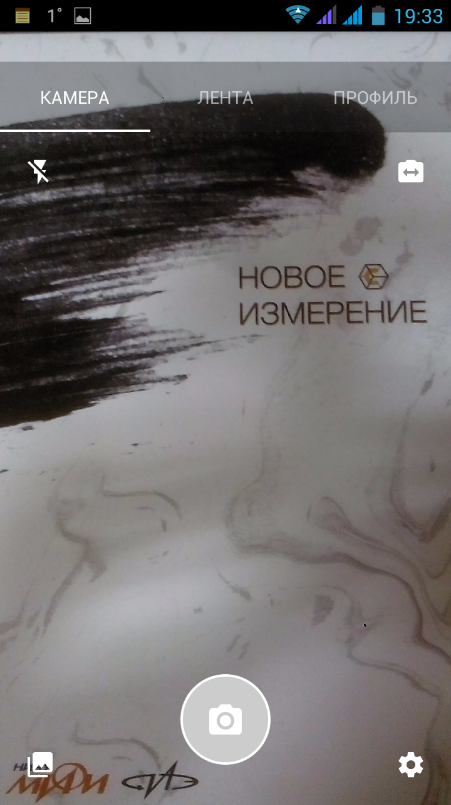
\includegraphics[width=0.3\linewidth]{pics/prismaCam}
	%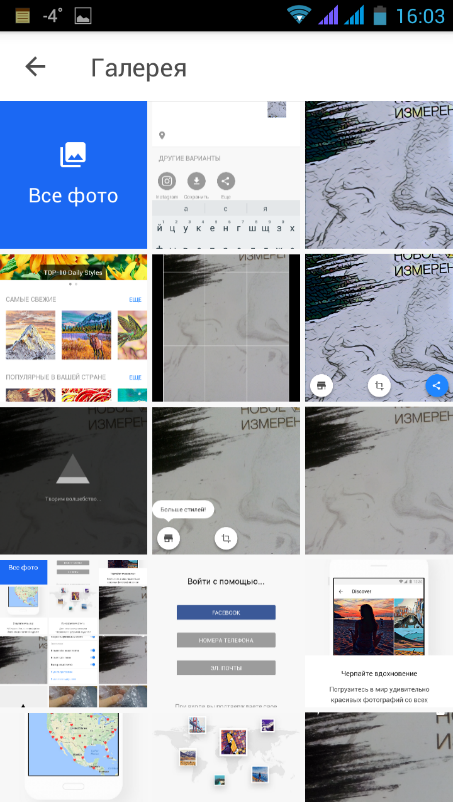
\includegraphics[width=0.3\linewidth]{pics/prismaGal}
	%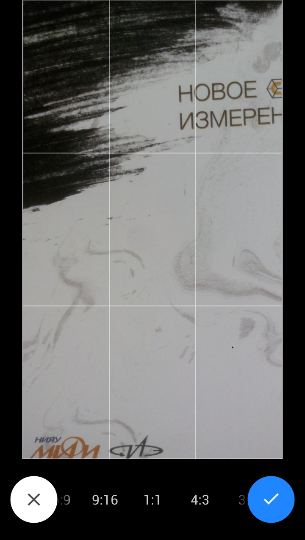
\includegraphics[width=0.3\linewidth]{pics/prismaProp}
	\caption{Prisma, окно с камерой}
	\label{fig:prismaCam}
	\label{fig:prismaGal}
	\label{fig:prismaProp}
\end{figure}

\begin{figure}[H]
	\centering
	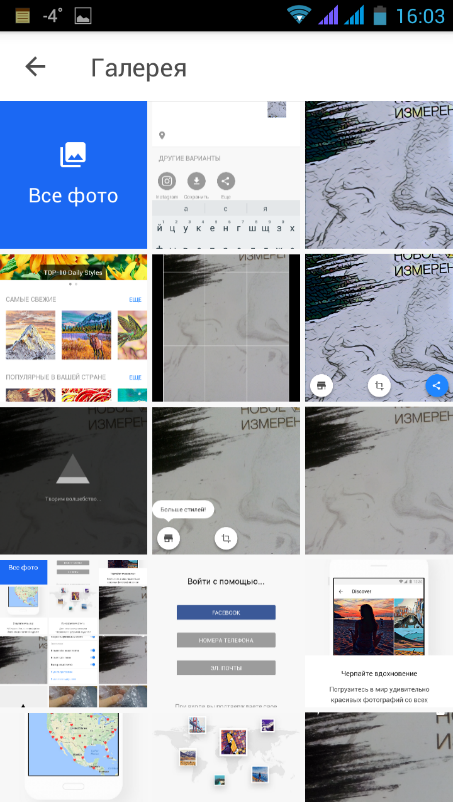
\includegraphics[width=0.3\linewidth]{pics/prismaGal}
	\caption{Prisma, окно с галереей}
	\label{fig:prismaGal}
\end{figure}

\begin{figure}[H]
	\centering
	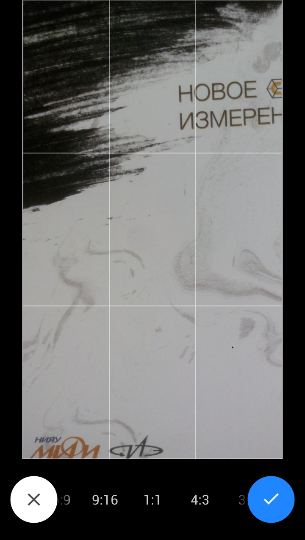
\includegraphics[width=0.3\linewidth]{pics/prismaProp}
	\caption{Prisma, окно выбора пропорции для изображения}
	\label{fig:prismaProp}
\end{figure}

\subsection{Candy Camera}
Проанализировав пользовательский интерфейс приложения Candy Camera (рисунок ~\ref{fig:candyCam}), в режиме камеры видим большое количество кнопок, не все их назначения понятны с первого раза. Фильтры и соотношения фотографии применяются сразу в режиме камеры. Заметное отличие заключается в том, что, сделав фотографию есть 3 секунды чтобы выбрать кнопку поделиться с друзьями или удалить фото (рисунок ~\ref{fig:candyGal}). Не выбрав ничего продолжается режим фотографирования. После можно вернуться к сделанным фотографиям через галерею, потом применить фильтр и поделиться изображением в социальных сетях (рисунок ~\ref{fig:candyPod}). В галереи все изображения рассортированы по дням, в отдельных блоках.

\begin{figure}[H]
	\centering
	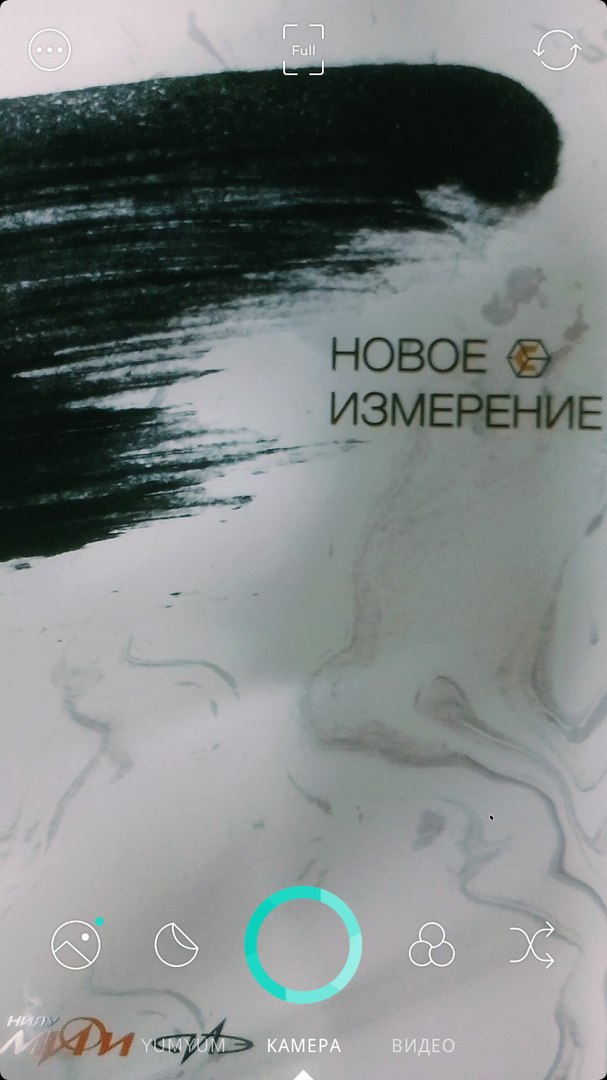
\includegraphics[width=0.3\linewidth]{pics/candyCam}
	\caption{Candy Camera, окно с камерой}
	\label{fig:candyCam}
\end{figure}

\begin{figure}[H]
	\centering
	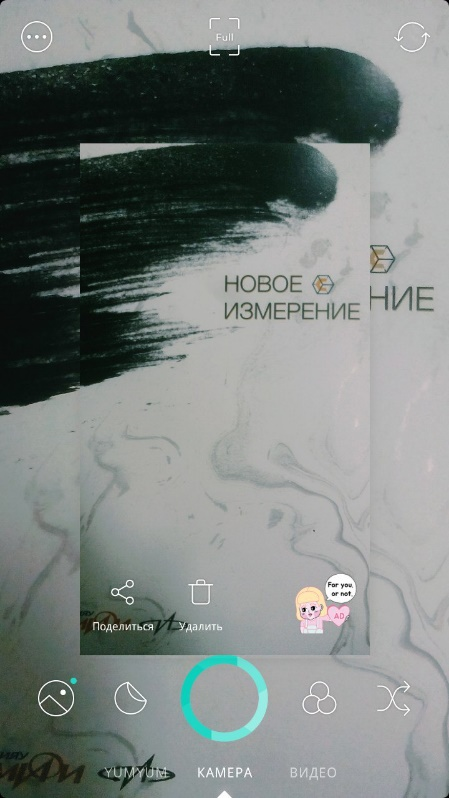
\includegraphics[width=0.3\linewidth]{pics/candyGal}
	\caption{Candy Camera, окно с просмотром фото}
	\label{fig:candyGal}
\end{figure}

\begin{figure}[H]
	\centering
	
\includegraphics[width=0.3\linewidth]{pics/candyPod}
	\caption{Candy Camera, окно выбора с кем поделиться изображением}
	\label{fig:candyPod}
\end{figure}

\subsection{Pixlr}
Проанализировав пользовательский интерфейс приложения Pixlr (рисунок ~\ref{fig:pixlrMenu}), основное различие с предыдущими приложениями это наличие главного меню, которое открывается при запуске программы. В меню можно выбрать дальнейшее действие, открыть камеру и сделать фотографию или открыть галерею и выбрать картинку из имеющихся изображений. Из режима камеры нельзя перейти в галерею (рисунок ~\ref{fig:pixlrCam}). Имеются кнопки с фильтрами, которые применяются сразу. Сделав фотографию, мы оцениваем ее и решаем сделать новое фото или продолжить редактировать. Галерея открывается с помощью стандартного просмоторщика галереи этого телефона. Применив фильтр, Pixlr предлагает запостить фото в разные социальные сети, сохранить изображение или выбор дополнительных действий с картинкой (рисунок ~\ref{fig:pixlrPod}). При сохранении можно выбрать разрешение, формат JPEG или PNG и качество изображения, после сохранения остается возможность поделиться этой фотографией в социальных сетях.

\begin{figure}[H]
	\centering
	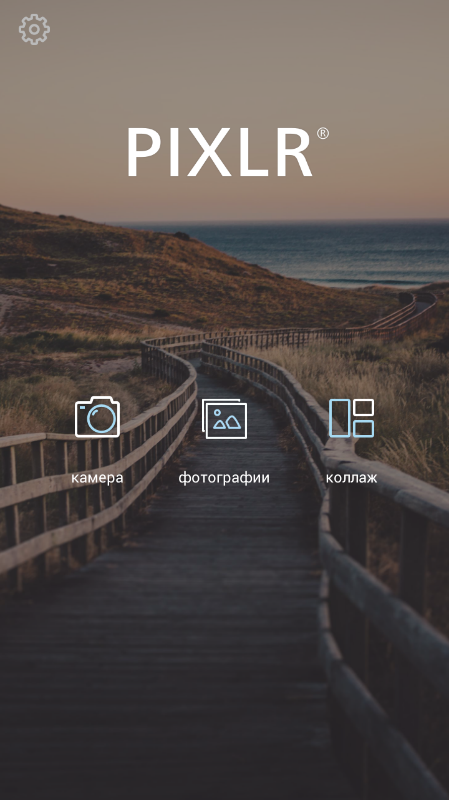
\includegraphics[width=0.3\linewidth]{pics/pixlrMenu}
	\caption{Pixlr, главное меню}
	\label{fig:pixlrMenu}
\end{figure}

\begin{figure}[H]
	\centering
	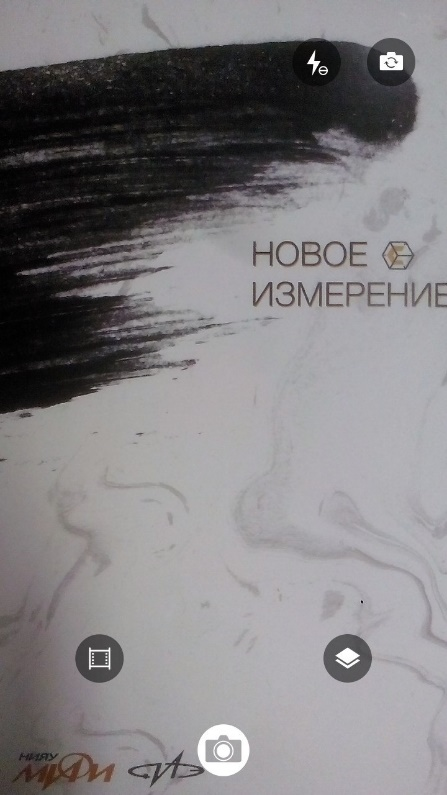
\includegraphics[width=0.3\linewidth]{pics/pixlrCam}
	\caption{Pixlr, окно с камерой}
	\label{fig:pixlrCam}
\end{figure}

\begin{figure}[H]
	\centering
	
\includegraphics[width=0.3\linewidth]{pics/pixlrPod}
	\caption{Pixlr, окно выбора с кем поделиться изображением}
	\label{fig:pixlrPod}
\end{figure}

\subsection{Анализ интерфейса}
Сравнив данные приложения, увидели общие черты, в режиме камеры имеются кнопки переключения режима фотовспышки и переключение между основной и фронтальной камерами. Есть возможность выбора соотношений, пропорций фотографии. Везде есть возможность поделиться фотографией в Instagram.

У Pixlr есть отличительная черта, это наличие главного меню и отсутствие собственного пользовательского интерфейса галереи. У Prisma, интерфейс галереи реализован лучше чем у Candy Camera. У Pixlr и Candy Camera есть удобная возможность просматривать фильтр в живую, еще не сделав фотографии. В режиме камеры у Pixlr и Prisma, кнопки расположены и выглядят более удобно чем у Candy Camera. Окно выбора действия с отредактированным изображением (сохранить или поделиться фотографией в социальных сетях) у Pixlr реализовано лучше.

Считаю, что необходимый набор функций программы должен включать: выбор фотографии из стандартной галереи, режим камеры, обработка изображения, просмотр результата, возможность сохранить, поделиться фотографией в социальных сетях и дополнительные возможности передачи картинки.

Необходимый набор элементов пользовательского интерфейса камеры должен включать: переключение режимов фотовспышки, переключение главной и фронтальной камеры, кнопку настроек, переход к выбору фотографии из галереи.

Мы планируем сделать приложение следующим образом, при включении откроется камера (рисунок ~\ref{fig:cam}), сделав фотографию пользователю предстоит оценить получившуюся фотографию и если нравится, то перейти к редактированию изображения, иначе сделать новое фото (рисунок ~\ref{fig:foto}). Сделав удовлетворяющую фотографию или выбрав нужную из галереи, происходит обработка изображения, и пользователь может просмотреть получившуюся картинку. Тут же есть возможность вернуться к камере, обрезать или продолжить. Выбрав продолжить, появляется окно с выбором дальнейших действий с данной фотографией, запостить фото в социальных сетях на выбор, сохранить изображение в пользовательском качестве или дополнительные способы передачи картинки (рисунок ~\ref{fig:pod}).

\begin{figure}[H]
	\centering
	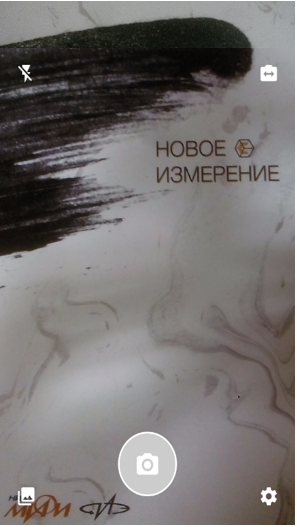
\includegraphics[width=0.3\linewidth]{pics/cam}
	\caption{Окно с камерой}
	\label{fig:cam}
\end{figure}

\begin{figure}[H]
	\centering
	
\includegraphics[width=0.3\linewidth]{pics/foto}
	\caption{Окно с просмотром фото}
	\label{fig:foto}
\end{figure}

\begin{figure}[H]
	\centering
	\includegraphics[width=0.3\linewidth]{pics/Pod}
	\caption{Окно выбора с кем поделиться изображением}
	\label{fig:Pod}
\end{figure}

При создании пользовательского интерфейса приложения были проанализированы современные, с аналогичным функционалом мобильные приложения в целом. Был сделан акцент на необходимости создания современного, функционального и не перегруженного пользовательского интерфейса. В результате проведенного анализа был создан пользовательский интерфейс мобильного приложения для преобразования 2D фотографий в 3D вид.

  % первая глава - в файле part1.tex
%\pagebreak
%% второй раздел - файл part2.tex

\section{Обработка результатов расчетов ПК SERPENT2}

Главной задачей на текущий семестр является создание скриптов, которые смогут помочь автоматизировать функции, необходимые для определения нуклидного состава ядерного топлива, который будет использоваться в качестве входных условий для SERPENT2. 

\subsection{Python-скрипт для поиска и извлечения информации из расчетных файлов}

После того, как была проанализорована структура расчетных файлов, можно начинать приступать к извлечению и анализу информации, которая в них содержится.

Для этого необходимо реализовать скрипты, которые могли бы:

\begin{enumerate}
	\item Осуществлять поиск конкретных видов топлива, в текстовом файле начальных условий.
	\item Получать данные о концентрации нуклидов конкретного топлива в выходном файле расчета выгорания.
\end{enumerate}

Для решения поставленных задач были реализованы скрипты на языке Python \cite{python}:

\begin{enumerate}
	\item Searher.py
	\item fuelGetter.py
\end{enumerate}

Класс Searcher.py содержит функцию, необходимые для поиска содержащихся видов топлива (fuel) в текстовом файле начальных условий (листинг ~\ref{fuelList}), а также  функцию, которая извлекает для каждого вида топлива данные об изменении концетрации нуклидов топлива во времени из файла расчета выгорания(листинг ~\ref{adens}). 

%Для отображения исходных кодов (см. пример ссылки на литературу \cite{Rrus1}) можно  воспользоваться окружением \verb|MyCode|:

%\begin{MyCode}
%require(ggplot2)
%gi = ggplot(data = iris, aes(x=Sepal.Length,y=Petal.Length))
%gi + geom_point(aes(color=Species))
%\end{MyCode}

%Для нумерации листингов и возможности ссылаться на них  предназначено окружение \verb|Program|.

\begin{Program}[H]
\begin{MyCode}
@staticmethod
def search_in_txt_file(filename):
"""метод ищет в строке, если есть burn соответствующий fuel и
формирует массив для посика соответствующего ADENS"""
f = open(filename, 'r')
l_burns = list() #создаем список строк для fuel - формата:
					 MAT_fuel ... _ADENS
subs = "fuel"
substr = "burn"
pattern_part1 = "MAT_"   # was 'MAT_fuel'
pattern_part2 = "_ADENS = ["
for line in f:  # для каждой строки из файла ищем
	if substr in line:  # если строка содержит слово burn
		s = line.split()  # разбиваем ее по пробелам
		for ss in s:  #для каждого элемента 
		разбиенной строки ещем
			if subs in ss: #содержит ли элемент
				подстроку fuel
			   hvost = ss[ss.rfind(subs): len(ss)]  
				#создаем переменную, которая
				 будет содержать 
				соответствующее число,
				 стоящее после fuel
		l_burns.append(pattern_part1 + hvost +
						 pattern_part2) 
		  # формируем строку формата: 
			 	MAT_fuel+hvost_ADENS

return l_burns
\end{MyCode}
\label{fuelList}
\caption{Функция получения списка видов топлива}
\end{Program}

\begin{Program}[H]
\begin{MyCode}
		@staticmethod
		def search_in_m_file(l_burns, filesPath, m_filename):
		"""Метод ищет в .m файле ADENS-ы и извлекает все, что
		находится между квадратными скобками, для каждого fuel"""
		last_symbol = "]"
		m_file = open(m_filename, 'r') #открываем .m файл для чтения 
		и нахождения соответствующих ADENS
		text = m_file.read()
		for l in l_burns:  #для каждого элемента массива, 
		содержащего паттерны ADENS
		if l in text:
		start = text.find(l)+ len(l)
		end = text.find(last_symbol, start)
		adens = text[start : end]
		filename = str(filesPath + l + ".txt")
		adens_file = open(filename, "w")
		adens_file.write(adens)
		adens_file.close()		
\end{MyCode}
\label{adens}
\caption{Функция извлечения данных об изменении концетрации нуклидов топлива во времени}
\end{Program}

А скрипт fuelGetter.py запускает фукнцию получения списка видов топлива и будет использоваться в Java-приложении.


\subsection{Реалиация Java-приложения}

\subsubsection{Стартовое окно}

Теперь, когда скрипты для извлечения данных о топливе и его видах получены, можно реализовать Java-приложение \cite{shild} для управления обработкой результатов расчетов SERPENT-а. 

При запуске приложения появляется следующее окно (рисунок ~\ref{fig:startWindow}):

\begin{figure}[H]
	\centering
	\includegraphics[width=0.5\linewidth]{pics/startWindow}
	\caption{Стартовое окно приложения}
	\label{fig:startWindow}
\end{figure}

Данное окно содержит активную кнопку, по нажатию которой можно получить список всех видов топлива из текстового файла. Иными словами, она запускает Python-скрипт fuelGetter.py и результаты его работы выводятся в окно Java-приложения.

Как только список видов топлива был получен, можно начать работать с конкретным видом. После выбора определенного вида топлива становятся активными еще 2 кнопки(рисунок ~\ref{fig:startActive}): "Получить информацию о виде топлива" и "Информация о концентрации вида топлива".

\begin{figure}[H]
	\centering
	\includegraphics[width=0.5\linewidth]{pics/startActive}
	\caption{Начало работы с конкретным видом топлива}
	\label{fig:startActive}
\end{figure}

\subsubsection{Получение информации о виде топлива}

При нажатии на кнопку  "Получить информацию о виде топлива" пользователь получает полный список нуклидов, из которых состоит выбранный вид топлива:

\begin{figure}[H]
	\centering
	\includegraphics[width=0.5\linewidth]{pics/nuclides}
	\caption{Начало работы с конкретным видом топлива}
	\label{fig:nuclides}
\end{figure}

По каждому нуклиду можно будет просмотреть изменение его концентраций, при нажатии соответствующей кнопки (рисунки ~\ref{fig:nuclideList}, ~\ref{fig:nuclideList2}):

\begin{figure}[H]
	\centering
	\includegraphics[width=0.5\linewidth]{pics/nuclideList}
	\caption{Начало работы с конкретным видом топлива}
	\label{fig:nuclideList}
\end{figure}

\begin{figure}[H]
	\centering
	\includegraphics[width=0.5\linewidth]{pics/nuclideList2}
	\caption{Начало работы с конкретным видом топлива}
	\label{fig:nuclideList2}
\end{figure}

Также, выбранный нуклид можно удалить из списка нуклидов, составляющих топливо.

\subsubsection{Получение информации о концентрации вида топлива} 

Если же пользователю хочется увидеть изменение концентраций всех нуклидов и выбрать определенный столбец концентраций в качестве начальных условий для данного вида топлива, то в стартовом окне ему необходимо нажать на кнопку "Информация о концентрации вида топлива". Необходимая информация появится в таблице (рисунок  ~\ref{fig:table}). 

\begin{figure}[H]
	\centering
	\includegraphics[width=0.9\linewidth]{pics/table}
	\caption{Изменение концентраций всех нуклидов во времени}
	\label{fig:table}
\end{figure}

Любой из столбцов таблицы может быть выбран в качестве начальных условий для данного вида топлива(начальные условия описываются в текстовом файле). Для этого пользователь может нажать на кнопку <<Сделать начальным условием>> и указанный пользователем столбец будет запишется в новый текстовый файл начальных условий как показано на рисунке ниже:

\begin{figure}[H]
	\centering
	\includegraphics[width=0.5\linewidth]{pics/newtxt}
	\caption{Текстовый файл начальных условий}
	\label{fig:newtxt}
\end{figure}

Эти же выбранные начальные условия можно отобразить на графике с использованием логарифмической шкалы. Для этого необходимо перейти по кнопке <<Изобразить>>. 

\begin{figure}[H]
	\centering
	\includegraphics[width=0.5\linewidth]{pics/diagram}
	\caption{Пример динамики концентрации радионуклида}
	\label{fig:diagram}
\end{figure}

%Следует учесть, что объем кода в таком листинге должен быть небольшим --- меньше страницы, а нумерация появляется, если внутри окружения задано название листинга с помощью команды \verb|\caption|. 

%Кроме того, положение кода выбирается системой \LaTeXe.
%\pagebreak

\pagebreak
\section*{\centering ЗАКЛЮЧЕНИЕ}
\addcontentsline{toc}{section}{ЗАКЛЮЧЕНИЕ}
В ходе проделанной работы были исследованы методы  метода «дефокусировки» и семантического анализа.

При создании пользовательского интерфейса приложения были проанализированы современные, с аналогичным функционалом мобильные приложения в целом. Был сделан акцент на необходимости создания современного, функционального и не перегруженного пользовательского интерфейса. В результате проведенного анализа был создан пользовательский интерфейс мобильного приложения для преобразования 2D фотографий в 3D вид.

% оформление библиографии - вариант с БД

\pagebreak
\addcontentsline{toc}{section}{СПИСОК ИСПОЛЬЗОВАННОЙ ЛИТЕРАТУРЫ}
\printbibliography

%\pagebreak
%\section*{\centering Приложение А}
%\addcontentsline{toc}{section}{Приложение А}
%приложение А

%\pagebreak
%\section*{\centering Приложение Б}
%\addcontentsline{toc}{section}{Приложение Б}
%приложение Б

\end{document}          

